% Options for packages loaded elsewhere
\PassOptionsToPackage{unicode}{hyperref}
\PassOptionsToPackage{hyphens}{url}
%
\documentclass[
]{article}
\usepackage{amsmath,amssymb}
\usepackage{iftex}
\ifPDFTeX
  \usepackage[T1]{fontenc}
  \usepackage[utf8]{inputenc}
  \usepackage{textcomp} % provide euro and other symbols
\else % if luatex or xetex
  \usepackage{unicode-math} % this also loads fontspec
  \defaultfontfeatures{Scale=MatchLowercase}
  \defaultfontfeatures[\rmfamily]{Ligatures=TeX,Scale=1}
\fi
\usepackage{lmodern}
\ifPDFTeX\else
  % xetex/luatex font selection
\fi
% Use upquote if available, for straight quotes in verbatim environments
\IfFileExists{upquote.sty}{\usepackage{upquote}}{}
\IfFileExists{microtype.sty}{% use microtype if available
  \usepackage[]{microtype}
  \UseMicrotypeSet[protrusion]{basicmath} % disable protrusion for tt fonts
}{}
\makeatletter
\@ifundefined{KOMAClassName}{% if non-KOMA class
  \IfFileExists{parskip.sty}{%
    \usepackage{parskip}
  }{% else
    \setlength{\parindent}{0pt}
    \setlength{\parskip}{6pt plus 2pt minus 1pt}}
}{% if KOMA class
  \KOMAoptions{parskip=half}}
\makeatother
\usepackage{xcolor}
\usepackage[margin=1in]{geometry}
\usepackage{color}
\usepackage{fancyvrb}
\newcommand{\VerbBar}{|}
\newcommand{\VERB}{\Verb[commandchars=\\\{\}]}
\DefineVerbatimEnvironment{Highlighting}{Verbatim}{commandchars=\\\{\}}
% Add ',fontsize=\small' for more characters per line
\usepackage{framed}
\definecolor{shadecolor}{RGB}{248,248,248}
\newenvironment{Shaded}{\begin{snugshade}}{\end{snugshade}}
\newcommand{\AlertTok}[1]{\textcolor[rgb]{0.94,0.16,0.16}{#1}}
\newcommand{\AnnotationTok}[1]{\textcolor[rgb]{0.56,0.35,0.01}{\textbf{\textit{#1}}}}
\newcommand{\AttributeTok}[1]{\textcolor[rgb]{0.13,0.29,0.53}{#1}}
\newcommand{\BaseNTok}[1]{\textcolor[rgb]{0.00,0.00,0.81}{#1}}
\newcommand{\BuiltInTok}[1]{#1}
\newcommand{\CharTok}[1]{\textcolor[rgb]{0.31,0.60,0.02}{#1}}
\newcommand{\CommentTok}[1]{\textcolor[rgb]{0.56,0.35,0.01}{\textit{#1}}}
\newcommand{\CommentVarTok}[1]{\textcolor[rgb]{0.56,0.35,0.01}{\textbf{\textit{#1}}}}
\newcommand{\ConstantTok}[1]{\textcolor[rgb]{0.56,0.35,0.01}{#1}}
\newcommand{\ControlFlowTok}[1]{\textcolor[rgb]{0.13,0.29,0.53}{\textbf{#1}}}
\newcommand{\DataTypeTok}[1]{\textcolor[rgb]{0.13,0.29,0.53}{#1}}
\newcommand{\DecValTok}[1]{\textcolor[rgb]{0.00,0.00,0.81}{#1}}
\newcommand{\DocumentationTok}[1]{\textcolor[rgb]{0.56,0.35,0.01}{\textbf{\textit{#1}}}}
\newcommand{\ErrorTok}[1]{\textcolor[rgb]{0.64,0.00,0.00}{\textbf{#1}}}
\newcommand{\ExtensionTok}[1]{#1}
\newcommand{\FloatTok}[1]{\textcolor[rgb]{0.00,0.00,0.81}{#1}}
\newcommand{\FunctionTok}[1]{\textcolor[rgb]{0.13,0.29,0.53}{\textbf{#1}}}
\newcommand{\ImportTok}[1]{#1}
\newcommand{\InformationTok}[1]{\textcolor[rgb]{0.56,0.35,0.01}{\textbf{\textit{#1}}}}
\newcommand{\KeywordTok}[1]{\textcolor[rgb]{0.13,0.29,0.53}{\textbf{#1}}}
\newcommand{\NormalTok}[1]{#1}
\newcommand{\OperatorTok}[1]{\textcolor[rgb]{0.81,0.36,0.00}{\textbf{#1}}}
\newcommand{\OtherTok}[1]{\textcolor[rgb]{0.56,0.35,0.01}{#1}}
\newcommand{\PreprocessorTok}[1]{\textcolor[rgb]{0.56,0.35,0.01}{\textit{#1}}}
\newcommand{\RegionMarkerTok}[1]{#1}
\newcommand{\SpecialCharTok}[1]{\textcolor[rgb]{0.81,0.36,0.00}{\textbf{#1}}}
\newcommand{\SpecialStringTok}[1]{\textcolor[rgb]{0.31,0.60,0.02}{#1}}
\newcommand{\StringTok}[1]{\textcolor[rgb]{0.31,0.60,0.02}{#1}}
\newcommand{\VariableTok}[1]{\textcolor[rgb]{0.00,0.00,0.00}{#1}}
\newcommand{\VerbatimStringTok}[1]{\textcolor[rgb]{0.31,0.60,0.02}{#1}}
\newcommand{\WarningTok}[1]{\textcolor[rgb]{0.56,0.35,0.01}{\textbf{\textit{#1}}}}
\usepackage{longtable,booktabs,array}
\usepackage{calc} % for calculating minipage widths
% Correct order of tables after \paragraph or \subparagraph
\usepackage{etoolbox}
\makeatletter
\patchcmd\longtable{\par}{\if@noskipsec\mbox{}\fi\par}{}{}
\makeatother
% Allow footnotes in longtable head/foot
\IfFileExists{footnotehyper.sty}{\usepackage{footnotehyper}}{\usepackage{footnote}}
\makesavenoteenv{longtable}
\usepackage{graphicx}
\makeatletter
\def\maxwidth{\ifdim\Gin@nat@width>\linewidth\linewidth\else\Gin@nat@width\fi}
\def\maxheight{\ifdim\Gin@nat@height>\textheight\textheight\else\Gin@nat@height\fi}
\makeatother
% Scale images if necessary, so that they will not overflow the page
% margins by default, and it is still possible to overwrite the defaults
% using explicit options in \includegraphics[width, height, ...]{}
\setkeys{Gin}{width=\maxwidth,height=\maxheight,keepaspectratio}
% Set default figure placement to htbp
\makeatletter
\def\fps@figure{htbp}
\makeatother
\setlength{\emergencystretch}{3em} % prevent overfull lines
\providecommand{\tightlist}{%
  \setlength{\itemsep}{0pt}\setlength{\parskip}{0pt}}
\setcounter{secnumdepth}{5}
\ifLuaTeX
  \usepackage{selnolig}  % disable illegal ligatures
\fi
\usepackage{bookmark}
\IfFileExists{xurl.sty}{\usepackage{xurl}}{} % add URL line breaks if available
\urlstyle{same}
\hypersetup{
  pdftitle={Walkthrough for the CLVTools Package},
  hidelinks,
  pdfcreator={LaTeX via pandoc}}

\title{Walkthrough for the CLVTools Package}
\author{}
\date{\vspace{-2.5em}}

\begin{document}
\maketitle

{
\setcounter{tocdepth}{2}
\tableofcontents
}
\section{Prerequisites: Setup the R
environment}\label{prerequisites-setup-the-r-environment}

Install the stable version from CRAN:

\begin{Shaded}
\begin{Highlighting}[]
\FunctionTok{install.packages}\NormalTok{(}\StringTok{"CLVTools"}\NormalTok{)}
\end{Highlighting}
\end{Shaded}

Install the development version from GitHub (using the \texttt{devtools}
package {[}@devtools{]}):

Load the package

\begin{Shaded}
\begin{Highlighting}[]
\FunctionTok{library}\NormalTok{(}\StringTok{"CLVTools"}\NormalTok{)}
\end{Highlighting}
\end{Shaded}

\section{\texorpdfstring{Apply the \texttt{CLVTools}
Package}{Apply the CLVTools Package}}\label{apply-the-clvtools-package}

\subsection{General workflow}\label{general-workflow}

Independent of the latent attrition model applied in \texttt{CLVTools},
the general workflow consists of three main steps:

\begin{enumerate}
\def\labelenumi{\arabic{enumi}.}
\item
  Create a \texttt{clv.data} object containing the dataset and required
  meta-information such as date formats and column names in the dataset.
  After initializing the object, there is the option to add additional
  information on covariates in a separate step.
\item
  Fit the model on the data provided.
\item
  Use the estimated model parameters to predict future customer purchase
  behavior.
\end{enumerate}

\begin{figure}
\centering
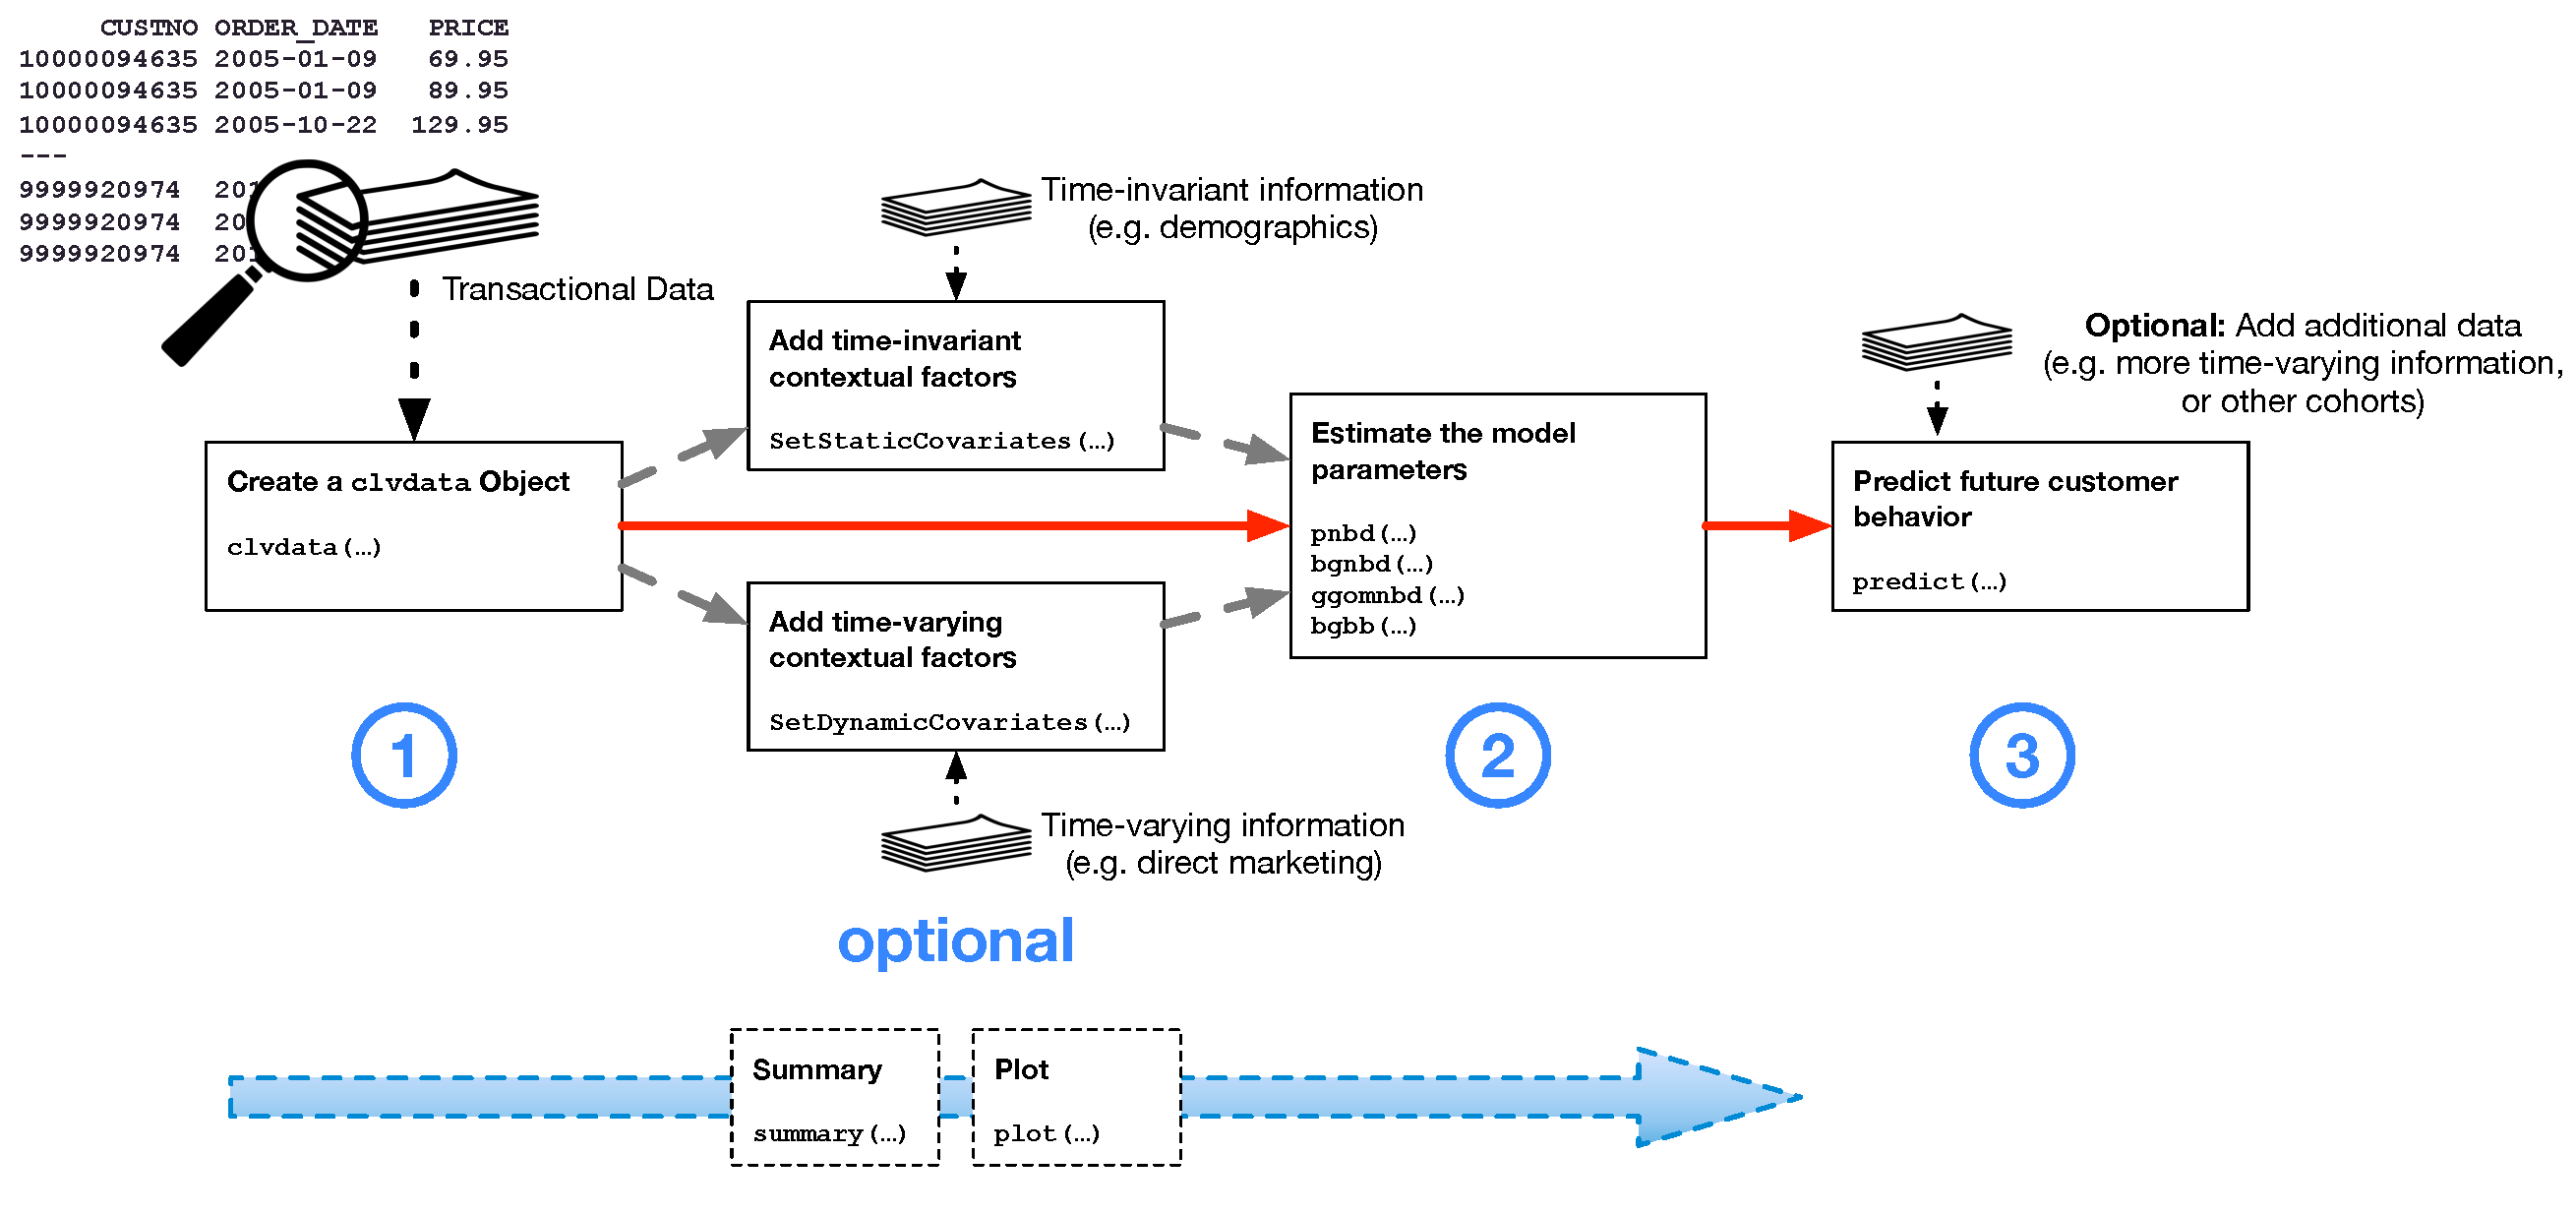
\includegraphics{figures/WALKTHROUGH-steps.pdf}
\caption{Workflow for \texttt{CLVTools}}
\end{figure}

\texttt{CLVTools} provides two ways for evaluating latent attrition
models: you can use of the provided formula interface or you can use
standard functions (non-formula interface). Both offer the same
functionality, however the formula interface is especially helpful when
covariates are included in the model. Through out this walkthrough, we
will illustrate both options.

Reporting and plotting results is facilitated by the implementation of
well-known generic methods such as \texttt{plot()}, \texttt{print()} and
\texttt{summary()}. These commands adapt their output according to the
model state and may be used at any point of the workflow.

\subsection{Load sample data provided in the
package}\label{load-sample-data-provided-in-the-package}

As Input data \texttt{CLVTools} requires customers' transaction history.
Every transaction record consists of a purchase date and customer ID.
Optionally, the price of the transaction may be included to allow for
prediction of future customer spending using an additional Gamma/Gamma
model{[}@Fader2005b; @Colombo1999{]}. Using the full history of
transaction data allows for comprehensive plots and summary statistics,
which allow the identification of possible issues prior to model
estimation. Data may be provided as \texttt{data.frame} or
\texttt{data.table} {[}@data.table{]}.

It is common practice to split time series data into two parts, an
estimation and a holdout period. The model is estimated based on the
data from the estimation period while the data from the holdout period
allows to rigorously assess model performance. Once model performance is
checked on known data one can proceed to predict data without a holdout
period. The length of the estimation period is heavily dependent on the
characteristics of the analyzed dataset. We recommend to choose an
estimation period that contains in minimum the length of the average
inter-purchase time. Note that all customers in the dataset need to
purchase at least once during the estimation period, i.e.~these models
do not account for prospects who have not yet a purchase record.

Some models included in \texttt{CLVTools} allow to model the impact of
covariates. These covariates may explain heterogeneity among the
customers and therefore increase the predictive accuracy of the model.
At the same time, we may also identify and quantify the effects of these
covariates on customer purchase and customer attrition.
\texttt{CLVTools} distinguishes between time-invariant and time-varying
covariates. Time-invariant covariates include customer characteristics
such as demographics that do not change over time. Time-varying
covariates are allowed to change over time. They include for example
direct marketing information or seasonal patterns.

For the following example, we use simulated data comparable to data from
a retailer in the apparel industry. The dataset contains transactional
detail records for every customer consisting of customer id, date of
purchase and the total monetary value of the transaction. The apparel
dataset is available in the \texttt{CLVTools} package. Use the
\texttt{data(apparelTrans)} to load it:

\begin{Shaded}
\begin{Highlighting}[]
\FunctionTok{data}\NormalTok{(}\StringTok{"apparelTrans"}\NormalTok{)}
\NormalTok{apparelTrans}
\CommentTok{\#\textgreater{}           Id       Date  Price}
\CommentTok{\#\textgreater{}       \textless{}char\textgreater{}     \textless{}Date\textgreater{}  \textless{}num\textgreater{}}
\CommentTok{\#\textgreater{}    1:      1 2005{-}01{-}02 230.30}
\CommentTok{\#\textgreater{}    2:      1 2005{-}09{-}06  84.39}
\CommentTok{\#\textgreater{}    3:      1 2006{-}01{-}18 131.07}
\CommentTok{\#\textgreater{}    4:      1 2006{-}04{-}05  86.43}
\CommentTok{\#\textgreater{}    5:      1 2006{-}07{-}02  11.49}
\CommentTok{\#\textgreater{}   {-}{-}{-}                         }
\CommentTok{\#\textgreater{} 3183:    600 2005{-}01{-}02  24.94}
\CommentTok{\#\textgreater{} 3184:    600 2005{-}04{-}17  54.97}
\CommentTok{\#\textgreater{} 3185:    600 2005{-}06{-}30  66.84}
\CommentTok{\#\textgreater{} 3186:    600 2005{-}10{-}27  22.54}
\CommentTok{\#\textgreater{} 3187:    600 2006{-}01{-}09  12.97}
\end{Highlighting}
\end{Shaded}

\subsection{Initialize the CLV-Object}\label{clvdata}

Before we estimate a model, we are required to initialize a data object
using the \texttt{clvdata()} command. The data object contains the
prepared transactional data and is later used as input for model
fitting. Make sure to store the generated object in a variable, e.g.~in
our example \texttt{clv.apparel}.

Be aware that probabilistic models such as the ones implemented in
\texttt{CLVTools} are usually applied to specific customer cohorts. That
means, you analyze customer that have joined your company at the same
time (usually same day, week, month, or quarter). For more information
on cohort analysis, see also
\href{https://en.wikipedia.org/wiki/Cohort_analysis}{here}.
Consequently, the data apparelTrans in this example is not the full
transaction records of a fashion retailer, but rather only the customer
cohort of 250 customers purchasing for the first time at this business
on the day of 2005-01-03. This has to be done before initializing a data
object using the \texttt{clvdata()} command.

Through the argument \texttt{data.transactions} a \texttt{data.frame} or
\texttt{data.table} which contains the transaction records, is
specified. In our example this is
\texttt{data.transactions=apparelTrans}. The argument
\texttt{date.format} is used to indicate the format of the date variable
in the data used. The date format in the apparel dataset is given as
``year-month-day'' (i.e., ``2005-01-03''), therefore we set
\texttt{date.format="ymd"}. Other combinations such as
\texttt{date.format="dmy"} are possible. See the documentation of
\texttt{lubridate} {[}@lubridate{]} for all details. \texttt{time.unit}
is the scale used to measure time between two dates. For this dataset
and in most other cases The argument \texttt{time.unit="week"} is the
preferred choice. Abbreviations may be used (i.e.~``w'').
\texttt{estimation.split} indicates the length of the estimation period.
Either the length of the estimation period (in previous specified time
units) or the date at which the estimation period ends can be specified.
If no value is provided, the whole dataset is used as estimation period
(i.e.~no holdout period). In this example, we use an estimation period
of 40 weeks. Finally, the three name arguments indicate the column names
for customer ID, date and price in the supplied dataset. Note that the
price column is optional.

\begin{Shaded}
\begin{Highlighting}[]
\NormalTok{clv.apparel }\OtherTok{\textless{}{-}} \FunctionTok{clvdata}\NormalTok{(apparelTrans,  }
                       \AttributeTok{date.format=}\StringTok{"ymd"}\NormalTok{, }
                       \AttributeTok{time.unit =} \StringTok{"week"}\NormalTok{,}
                       \AttributeTok{estimation.split =} \DecValTok{104}\NormalTok{,}
                       \AttributeTok{name.id =} \StringTok{"Id"}\NormalTok{,}
                       \AttributeTok{name.date =} \StringTok{"Date"}\NormalTok{,}
                       \AttributeTok{name.price =} \StringTok{"Price"}\NormalTok{)}
\end{Highlighting}
\end{Shaded}

\subsection{\texorpdfstring{Check the \texttt{clvdata}
Object}{Check the clvdata Object}}\label{check-the-clvdata-object}

To get details on the \texttt{clvdata} object, print it to the console.

\begin{Shaded}
\begin{Highlighting}[]
\NormalTok{clv.apparel}
\CommentTok{\#\textgreater{} CLV Transaction Data }
\CommentTok{\#\textgreater{} }
\CommentTok{\#\textgreater{} Call:}
\CommentTok{\#\textgreater{} clvdata(data.transactions = apparelTrans, date.format = "ymd", }
\CommentTok{\#\textgreater{}     time.unit = "week", estimation.split = 104, name.id = "Id", }
\CommentTok{\#\textgreater{}     name.date = "Date", name.price = "Price")}
\CommentTok{\#\textgreater{}                          }
\CommentTok{\#\textgreater{} Total \# customers    600 }
\CommentTok{\#\textgreater{} Total \# transactions 3183}
\CommentTok{\#\textgreater{} Spending information TRUE}
\CommentTok{\#\textgreater{} }
\CommentTok{\#\textgreater{}                                 }
\CommentTok{\#\textgreater{} Time unit         Weeks         }
\CommentTok{\#\textgreater{}                                 }
\CommentTok{\#\textgreater{} Estimation start  2005{-}01{-}02    }
\CommentTok{\#\textgreater{} Estimation end    2006{-}12{-}31    }
\CommentTok{\#\textgreater{} Estimation length 104.0000 Weeks}
\CommentTok{\#\textgreater{}                                 }
\CommentTok{\#\textgreater{} Holdout start     2007{-}01{-}01    }
\CommentTok{\#\textgreater{} Holdout end       2010{-}12{-}20    }
\CommentTok{\#\textgreater{} Holdout length    207.0000 Weeks}
\end{Highlighting}
\end{Shaded}

Alternatively the \texttt{summary()} command provides full detailed
summary statistics for the provided transactional detail.
\texttt{summary()} is available at any step in the process of estimating
a probabilistic customer attrition model with \texttt{CLVTools}. The
result output is updated accordingly and additional information is added
to the summary statistics.\texttt{nobs()} extracts the number of
observations. For the this particular dataset we observe a total of 250
customers who made in total 2257 repeat purchases. Approximately 26\% of
the customers are zero repeaters, which means that the only a minority
of the customers do not return to the store after their first purchase.

\begin{Shaded}
\begin{Highlighting}[]
\FunctionTok{summary}\NormalTok{(clv.apparel)}
\CommentTok{\#\textgreater{} CLV Transaction Data }
\CommentTok{\#\textgreater{}                                 }
\CommentTok{\#\textgreater{} Time unit         Weeks         }
\CommentTok{\#\textgreater{} Estimation length 104.0000 Weeks}
\CommentTok{\#\textgreater{} Holdout length    207.0000 Weeks}
\CommentTok{\#\textgreater{} }
\CommentTok{\#\textgreater{} Transaction Data Summary }
\CommentTok{\#\textgreater{}                                    Estimation      Holdout         Total     }
\CommentTok{\#\textgreater{} Period Start                       2005{-}01{-}02      2007{-}01{-}01      2005{-}01{-}02}
\CommentTok{\#\textgreater{} Period End                         2006{-}12{-}31      2010{-}12{-}20      2010{-}12{-}20}
\CommentTok{\#\textgreater{} Number of customers                {-}               {-}               600       }
\CommentTok{\#\textgreater{} First Transaction in period        2005{-}01{-}02      2007{-}01{-}01      2005{-}01{-}02}
\CommentTok{\#\textgreater{} Last Transaction in period         2006{-}12{-}31      2010{-}12{-}20      2010{-}12{-}20}
\CommentTok{\#\textgreater{} Total \# Transactions               1866            1317            3183      }
\CommentTok{\#\textgreater{} Mean \# Transactions per cust       3.110           5.557           5.305     }
\CommentTok{\#\textgreater{} (SD)                               2.714           5.123           6.119     }
\CommentTok{\#\textgreater{} Mean Spending per Transaction      40.545          36.977          39.069    }
\CommentTok{\#\textgreater{} (SD)                               73.362          55.356          66.519    }
\CommentTok{\#\textgreater{} Total Spending                     75657.730       48699.170       124356.900}
\CommentTok{\#\textgreater{} Total \# zero repeaters             213             {-}               {-}         }
\CommentTok{\#\textgreater{} Percentage of zero repeaters       35.500          {-}               {-}         }
\CommentTok{\#\textgreater{} Mean Interpurchase time            24.823          30.604          37.817    }
\CommentTok{\#\textgreater{} (SD)                               19.417          24.756          42.339}
\end{Highlighting}
\end{Shaded}

\subsection{Estimate Model Parameters}\label{estimate}

After initializing the object, we can start estimating the first
probabilistic latent attrition model. We start with the standard
Pareto/NBD model {[}@Schmittlein1987{]} and therefore use the command
\texttt{pnbd()} to fit the model and estimate model parameters.
\texttt{clv.data} specifies the initialized object prepared in the last
step. Optionally, starting values for the model parameters and control
settings for the optimization algorithm may be provided: The argument
\texttt{start.params.model} allows to assign a vector
(e.g.~\texttt{c(alpha=1,\ beta=2,\ s=1,\ beta=2)} in the case of the
Pareto/NBD model) of starting values for the optimization. This is
useful if prior knowledge on the parameters of the distributions are
available. By default starting values are set to 1 for all parameters.
The argument \texttt{optimx.args} provides an option to control settings
for the optimization routine. It passes a list of arguments to the
optimizer. All options known from the package \texttt{optimx}
{[}@optimx1; @optimx2{]} may be used. This option enables users to
specify specific optimization algorithms, set upper and/or lower limits
or enable tracing information on the progress of the optimization. In
the case of the standard Pareto/NBD model, \texttt{CLVTools} uses by
default the optimization method \texttt{L-BFGS-G}
{[}@byrd1995limited{]}. If the result of the optimization is
in-feasible, the optimization automatically switches to the more robust
but often slower \texttt{Nelder-Mead} method {[}@nelder1965simplex{]}.
\texttt{verbose} shows additional output.

To execute the model estimation you have the choice between a
formula-based interface and a non-formula-based interface. In the
following we illustrate the two alternatives.

\subsubsection{\texorpdfstring{\textbf{Estimating the model using
formula
interface:}}{Estimating the model using formula interface:}}\label{estimating-the-model-using-formula-interface}

\begin{Shaded}
\begin{Highlighting}[]
\NormalTok{   est.pnbd }\OtherTok{\textless{}{-}} \FunctionTok{latentAttrition}\NormalTok{(}\AttributeTok{formula =}\NormalTok{ , }\AttributeTok{family =}\NormalTok{ pnbd, }\AttributeTok{data=}\NormalTok{clv.apparel)}
\CommentTok{\#\textgreater{} Starting estimation...}
\CommentTok{\#\textgreater{} Estimation finished!}
\NormalTok{   est.pnbd}
\CommentTok{\#\textgreater{} Pareto/NBD Standard Model}
\CommentTok{\#\textgreater{} }
\CommentTok{\#\textgreater{} Call:}
\CommentTok{\#\textgreater{} latentAttrition(family = pnbd, data = clv.apparel)}
\CommentTok{\#\textgreater{} }
\CommentTok{\#\textgreater{} Coefficients:}
\CommentTok{\#\textgreater{}       r    alpha        s     beta  }
\CommentTok{\#\textgreater{}  1.4490  48.6361   0.5613  46.8844  }
\CommentTok{\#\textgreater{} KKT1: TRUE }
\CommentTok{\#\textgreater{} KKT2: TRUE }
\CommentTok{\#\textgreater{} }
\CommentTok{\#\textgreater{} Used Options:}
\CommentTok{\#\textgreater{} Correlation:     FALSE}
\end{Highlighting}
\end{Shaded}

\begin{verbatim}
Using start parameters and other additional arguments for the optimzier:
\end{verbatim}

\begin{Shaded}
\begin{Highlighting}[]
\NormalTok{  est.pnbd }\OtherTok{\textless{}{-}} \FunctionTok{latentAttrition}\NormalTok{(}\AttributeTok{formula =}\NormalTok{ , }\AttributeTok{family =}\NormalTok{ pnbd, }\AttributeTok{data=}\NormalTok{clv.apparel, }
                              \AttributeTok{optimx.args =} \FunctionTok{list}\NormalTok{(}\AttributeTok{control=}\FunctionTok{list}\NormalTok{(}\AttributeTok{trace=}\DecValTok{5}\NormalTok{),}
                                       \AttributeTok{method=}\StringTok{"Nelder{-}Mead"}\NormalTok{), }
                              \AttributeTok{start.params.model=}\FunctionTok{c}\NormalTok{(}\AttributeTok{r=}\DecValTok{1}\NormalTok{, }\AttributeTok{alpha=}\DecValTok{10}\NormalTok{, }\AttributeTok{s=}\DecValTok{2}\NormalTok{, }\AttributeTok{beta=}\DecValTok{8}\NormalTok{))}
\end{Highlighting}
\end{Shaded}

\subsubsection{\texorpdfstring{\textbf{Estimating the model using
non-formula
interface:}}{Estimating the model using non-formula interface:}}\label{estimating-the-model-using-non-formula-interface}

\begin{Shaded}
\begin{Highlighting}[]
\NormalTok{    est.pnbd }\OtherTok{\textless{}{-}} \FunctionTok{pnbd}\NormalTok{(}\AttributeTok{clv.data =}\NormalTok{ clv.apparel)}
\NormalTok{    est.pnbd}
\end{Highlighting}
\end{Shaded}

\begin{verbatim}
If we assign starting parameters and additional arguments for the optimizer we use: 
\end{verbatim}

\begin{Shaded}
\begin{Highlighting}[]
\NormalTok{   est.pnbd }\OtherTok{\textless{}{-}} \FunctionTok{pnbd}\NormalTok{(}\AttributeTok{clv.data =}\NormalTok{ clv.apparel, }
                    \AttributeTok{start.params.model =} \FunctionTok{c}\NormalTok{(}\AttributeTok{r=}\DecValTok{1}\NormalTok{, }\AttributeTok{alpha =} \DecValTok{2}\NormalTok{, }\AttributeTok{s =} \DecValTok{1}\NormalTok{, }\AttributeTok{beta =} \DecValTok{2}\NormalTok{), }
                    \AttributeTok{optimx.args =} \FunctionTok{list}\NormalTok{(}\AttributeTok{control=}\FunctionTok{list}\NormalTok{(}\AttributeTok{trace=}\DecValTok{5}\NormalTok{),}
                                       \AttributeTok{method=}\StringTok{"Nelder{-}Mead"} 
\NormalTok{                                       ))}
\end{Highlighting}
\end{Shaded}

Parameter estimates may be reported by either printing the estimated
object (i.e.~\texttt{est.pnbd}) directly in the console or by calling
\texttt{summary(est.pnbd)} to get a more detailed report including the
likelihood value as well as AIC and BIC. Alternatively parameters may be
directly extracted using \texttt{coef(est.pnbd)}. Also
\texttt{loglik()}, \texttt{confint()} and \texttt{vcov()} are available
to directly access the Loglikelihood value, confidence intervals for the
parameters and to calculate the Variance-Covariance Matrix for the
fitted model. For the standard Pareto/NBD model, we get 4 parameters
\(r, \alpha, s\) and \(\beta\). where \(r,\alpha\) represent the shape
and scale parameter of the gamma distribution that determines the
purchase rate and \(s,\beta\) of the attrition rate across individual
customers. \(r/\alpha\) can be interpreted as the mean purchase and
\(s/\beta\) as the mean attrition rate. A significance level is provided
for each parameter estimates. In the case of the apparelTrans dataset we
observe a an average purchase rate of \(r/\alpha=0.147\) transactions
and an average attrition rate of \(s/\beta=0.031\) per customer per
week. KKT 1 and 2 indicate the Karush-Kuhn-Tucker optimality conditions
of the first and second order {[}@KKT{]}. If those criteria are not met,
the optimizer has probably not arrived at an optimal solution. If this
is the case it is usually a good idea to rerun the estimation using
alternative starting values.

\begin{Shaded}
\begin{Highlighting}[]
\CommentTok{\#Full detailed summary of the parameter estimates}
\FunctionTok{summary}\NormalTok{(est.pnbd)}
\CommentTok{\#\textgreater{} Pareto/NBD Standard  Model }
\CommentTok{\#\textgreater{} }
\CommentTok{\#\textgreater{} Call:}
\CommentTok{\#\textgreater{} latentAttrition(family = pnbd, data = clv.apparel)}
\CommentTok{\#\textgreater{} }
\CommentTok{\#\textgreater{} Fitting period:                                }
\CommentTok{\#\textgreater{} Estimation start  2005{-}01{-}02    }
\CommentTok{\#\textgreater{} Estimation end    2006{-}12{-}31    }
\CommentTok{\#\textgreater{} Estimation length 104.0000 Weeks}
\CommentTok{\#\textgreater{} }
\CommentTok{\#\textgreater{} Coefficients:}
\CommentTok{\#\textgreater{}       Estimate Std. Error z{-}val Pr(\textgreater{}|z|)}
\CommentTok{\#\textgreater{} r       1.4490     0.2434    NA       NA}
\CommentTok{\#\textgreater{} alpha  48.6361     7.4892    NA       NA}
\CommentTok{\#\textgreater{} s       0.5613     0.2710    NA       NA}
\CommentTok{\#\textgreater{} beta   46.8844    35.6114    NA       NA}
\CommentTok{\#\textgreater{} }
\CommentTok{\#\textgreater{} Optimization info:                 }
\CommentTok{\#\textgreater{} LL     {-}5848.0978}
\CommentTok{\#\textgreater{} AIC    11704.1957}
\CommentTok{\#\textgreater{} BIC    11721.7834}
\CommentTok{\#\textgreater{} KKT 1  TRUE      }
\CommentTok{\#\textgreater{} KKT 2  TRUE      }
\CommentTok{\#\textgreater{} fevals 25.0000   }
\CommentTok{\#\textgreater{} Method L{-}BFGS{-}B  }
\CommentTok{\#\textgreater{} }
\CommentTok{\#\textgreater{} Used Options:                 }
\CommentTok{\#\textgreater{} Correlation FALSE}

\CommentTok{\#Extract the coefficients only}
\FunctionTok{coef}\NormalTok{(est.pnbd)}
\CommentTok{\#\textgreater{}          r      alpha          s       beta }
\CommentTok{\#\textgreater{}  1.4489768 48.6360846  0.5612598 46.8843631}
\CommentTok{\#Alternative: oefficients(est.pnbd.obj)}
\end{Highlighting}
\end{Shaded}

To extract only the coefficients, we can use \texttt{coef()}. To access
the confidence intervals for all parameters \texttt{confint()} is
available.

\begin{Shaded}
\begin{Highlighting}[]
\CommentTok{\#Extract the coefficients only}
\FunctionTok{coef}\NormalTok{(est.pnbd)}
\CommentTok{\#\textgreater{}          r      alpha          s       beta }
\CommentTok{\#\textgreater{}  1.4489768 48.6360846  0.5612598 46.8843631}
\CommentTok{\#Alternative: oefficients(est.pnbd.obj)}

\CommentTok{\#Extract the confidence intervals}
\FunctionTok{confint}\NormalTok{(est.pnbd)}
\CommentTok{\#\textgreater{}              2.5 \%     97.5 \%}
\CommentTok{\#\textgreater{} r       0.97186638   1.926087}
\CommentTok{\#\textgreater{} alpha  33.95755827  63.314611}
\CommentTok{\#\textgreater{} s       0.03001563   1.092504}
\CommentTok{\#\textgreater{} beta  {-}22.91272188 116.681448}
\end{Highlighting}
\end{Shaded}

In order to get the Likelihood value and the corresponding
Variance-Covariance Matrix we use the following commands:

\begin{Shaded}
\begin{Highlighting}[]
\CommentTok{\# LogLikelihood at maximum}
\FunctionTok{logLik}\NormalTok{(est.pnbd)}
\CommentTok{\#\textgreater{} \textquotesingle{}log Lik.\textquotesingle{} {-}5848.098 (df=4)}

\CommentTok{\# Variance{-}Covariance Matrix at maximum}
\FunctionTok{vcov}\NormalTok{(est.pnbd)}
\CommentTok{\#\textgreater{}                 r       alpha           s        beta}
\CommentTok{\#\textgreater{} r      0.05925727   1.7049763 {-}0.01786467   {-}3.472616}
\CommentTok{\#\textgreater{} alpha  1.70497628  56.0878419 {-}0.43375973  {-}82.963757}
\CommentTok{\#\textgreater{} s     {-}0.01786467  {-}0.4337597  0.07346698    9.366246}
\CommentTok{\#\textgreater{} beta  {-}3.47261649 {-}82.9637568  9.36624553 1268.172667}
\end{Highlighting}
\end{Shaded}

As an alternative to the Pareto/NBD model \texttt{CLVTools} features the
BG/NBD model {[}@Fader2005c{]} and the GGomp/NBD {[}@Bemmaor2012a{]}. To
use the alternative models replace \texttt{pnbd()} by the corresponding
model-command. Note that he naming and number of model parameters is
dependent on the model. Consult the manual for more details on the
individual models. Beside probabilistic latent attrition models,
\texttt{CLVTools} also features the Gamma/Gamma model {[}@Colombo1999;
@Fader2005c{]} which is used to predict customer spending. See section
\hyperref[spending]{Customer Spending} for details on the spending
model.

\begin{longtable}[]{@{}
  >{\raggedright\arraybackslash}p{(\columnwidth - 8\tabcolsep) * \real{0.2000}}
  >{\raggedright\arraybackslash}p{(\columnwidth - 8\tabcolsep) * \real{0.2000}}
  >{\raggedright\arraybackslash}p{(\columnwidth - 8\tabcolsep) * \real{0.2000}}
  >{\raggedright\arraybackslash}p{(\columnwidth - 8\tabcolsep) * \real{0.2000}}
  >{\raggedright\arraybackslash}p{(\columnwidth - 8\tabcolsep) * \real{0.2000}}@{}}
\toprule\noalign{}
\begin{minipage}[b]{\linewidth}\raggedright
Command
\end{minipage} & \begin{minipage}[b]{\linewidth}\raggedright
Model
\end{minipage} & \begin{minipage}[b]{\linewidth}\raggedright
Covariates
\end{minipage} & \begin{minipage}[b]{\linewidth}\raggedright
Type
\end{minipage} & \begin{minipage}[b]{\linewidth}\raggedright
\end{minipage} \\
\midrule\noalign{}
\endhead
\bottomrule\noalign{}
\endlastfoot
pnbd() & Pareto/NBD & time-invariant \& time-varying & latent attrition
model & \\
bgnbd() & BG/NBD & time-invariant & latent attrition model & \\
ggomnbd() & GGom/NBD & time-invariant & latent attrition model & \\
gg() & Gamma/Gamma & - & spending model & \\
\end{longtable}

To estimate the GGom/NBD model we apply the \texttt{ggomnbd()}to the
\texttt{clv.apparel} object. The GGom/NBD model is more flexible than
the Pareto/NBD model, however it sometimes is challenging to optimize.
Note that in this particular case providing start parameters is
essential to arrive at an optimal solution (i.e.~\texttt{kkt1:\ TRUE}
and \texttt{kkt2:\ TRUE}).

To execute the model estimation you have the choice between a
formula-based interface and a non-formula-based interface. In the
following we illustrate the two alternatives.

\subsubsection{\texorpdfstring{\textbf{Estimating the model using
formula
interface:}}{Estimating the model using formula interface:}}\label{estimating-the-model-using-formula-interface-1}

\begin{Shaded}
\begin{Highlighting}[]
\NormalTok{  est.ggomnbd }\OtherTok{\textless{}{-}} \FunctionTok{latentAttrition}\NormalTok{(}\AttributeTok{formula =}\NormalTok{ , }\AttributeTok{family =}\NormalTok{ ggomnbd, }\AttributeTok{data=}\NormalTok{clv.apparel, }
                                 \AttributeTok{optimx.args =} \FunctionTok{list}\NormalTok{(}\AttributeTok{method=}\StringTok{"Nelder{-}Mead"}\NormalTok{),}
                                 \AttributeTok{start.params.model=}\FunctionTok{c}\NormalTok{(}\AttributeTok{r=}\FloatTok{0.7}\NormalTok{, }\AttributeTok{alpha=}\DecValTok{5}\NormalTok{, }\AttributeTok{b=}\FloatTok{0.005}\NormalTok{,  }\AttributeTok{s=}\FloatTok{0.02}\NormalTok{, }\AttributeTok{beta=}\FloatTok{0.001}\NormalTok{))}
\end{Highlighting}
\end{Shaded}

\subsubsection{\texorpdfstring{\textbf{Estimating the model using
non-formula
interface:}}{Estimating the model using non-formula interface:}}\label{estimating-the-model-using-non-formula-interface-1}

\begin{Shaded}
\begin{Highlighting}[]
\NormalTok{est.ggomnbd }\OtherTok{\textless{}{-}} \FunctionTok{ggomnbd}\NormalTok{(}\AttributeTok{clv.data =}\NormalTok{ clv.apparel, }
                       \AttributeTok{start.params.model =} \FunctionTok{c}\NormalTok{(}\AttributeTok{r=}\FloatTok{0.7}\NormalTok{, }\AttributeTok{alpha=}\DecValTok{5}\NormalTok{, }\AttributeTok{b=}\FloatTok{0.005}\NormalTok{,  }\AttributeTok{s=}\FloatTok{0.02}\NormalTok{, }\AttributeTok{beta=}\FloatTok{0.001}\NormalTok{), }
                       \AttributeTok{optimx.args =} \FunctionTok{list}\NormalTok{(}\AttributeTok{method=}\StringTok{"Nelder{-}Mead"}\NormalTok{))}
\end{Highlighting}
\end{Shaded}

\subsection{Predict Customer Behavior}\label{predict}

Once the model parameters are estimated, we are able to predict future
customer behavior on an individual level. To do so, we use
\texttt{predict()} on the object with the estimated parameters
(i.e.~\texttt{est.pnbd}). The prediction period may be varied by
specifying \texttt{prediction.end}. It is possible to provide either an
end-date or a duration using the same time unit as specified when
initializing the object (i.e \texttt{prediction.end\ =\ "2006-05-08"} or
\texttt{prediction.end\ =\ 30}). By default, the prediction is made
until the end of the dataset specified in the \texttt{clvdata()}
command. The argument \texttt{continuous.discount.factor} allows to
adjust the discount rate used to estimated the discounted expected
transactions (DERT). The default value is \texttt{0.1} (=10\%). Make
sure to convert your discount rate if you use annual/monthly/weekly
discount rates. An annual rate of \texttt{(100\ x\ d)\textbackslash{}\%}
equals a continuous rate \texttt{delta\ =\ ln(1+d)}. To account for time
units which are not annual, the continuous rate has to be further
adjusted to \texttt{delta=ln(1+d)/k}, where \texttt{k} are the number of
time units in a year. Probabilistic customer attrition model predict in
general three expected characteristics for every customer:

\begin{itemize}
\tightlist
\item
  ``conditional expected transactions'' (CET), which is the number of
  transactions to expect form a customer during the prediction period,
\item
  ``probability of a customer being alive'' (PAlive) at the end of the
  estimation period and
\item
  ``discounted expected residual transactions'' (DERT) for every
  customer, which is the total number of transactions for the residual
  lifetime of a customer discounted to the end of the estimation period.
\end{itemize}

If spending information was provided when initializing the
\texttt{clvdata}-object, \texttt{CLVTools} provides prediction for

\begin{itemize}
\tightlist
\item
  predicted mean spending estimated by a Gamma/Gamma model
  {[}@Colombo1999; @Fader2005c{]} and
\item
  the customer lifetime value (CLV). CLV is calculated as the product of
  DERT and predicted spending.
\end{itemize}

If a holdout period is available additionally the true numbers of
transactions (``actual.x'') and true spending
(``actual.total.spending'') during the holdout period are reported.

To use the parameter estimates on new data (e.g., an other customer
cohort), the argument \texttt{newdata} optionally allows to provide a
new \texttt{clvdata} object.

\begin{Shaded}
\begin{Highlighting}[]
\NormalTok{results }\OtherTok{\textless{}{-}} \FunctionTok{predict}\NormalTok{(est.pnbd)}
\CommentTok{\#\textgreater{} Predicting from 2007{-}01{-}01 until (incl.) 2010{-}12{-}20 (207.14 Weeks).}
\CommentTok{\#\textgreater{} Estimating gg model to predict spending...}
\CommentTok{\#\textgreater{} Starting estimation...}
\CommentTok{\#\textgreater{} Estimation finished!}
\FunctionTok{print}\NormalTok{(results)}
\CommentTok{\#\textgreater{} Key: \textless{}Id\textgreater{}}
\CommentTok{\#\textgreater{}          Id period.first period.last period.length actual.x}
\CommentTok{\#\textgreater{}      \textless{}char\textgreater{}       \textless{}Date\textgreater{}      \textless{}Date\textgreater{}         \textless{}num\textgreater{}    \textless{}int\textgreater{}}
\CommentTok{\#\textgreater{}   1:      1   2007{-}01{-}01  2010{-}12{-}20      207.1429        0}
\CommentTok{\#\textgreater{}   2:     10   2007{-}01{-}01  2010{-}12{-}20      207.1429        1}
\CommentTok{\#\textgreater{}   3:    100   2007{-}01{-}01  2010{-}12{-}20      207.1429        9}
\CommentTok{\#\textgreater{}   4:    101   2007{-}01{-}01  2010{-}12{-}20      207.1429        0}
\CommentTok{\#\textgreater{}   5:    102   2007{-}01{-}01  2010{-}12{-}20      207.1429        0}
\CommentTok{\#\textgreater{}  {-}{-}{-}                                                       }
\CommentTok{\#\textgreater{} 596:     95   2007{-}01{-}01  2010{-}12{-}20      207.1429        4}
\CommentTok{\#\textgreater{} 597:     96   2007{-}01{-}01  2010{-}12{-}20      207.1429        3}
\CommentTok{\#\textgreater{} 598:     97   2007{-}01{-}01  2010{-}12{-}20      207.1429        0}
\CommentTok{\#\textgreater{} 599:     98   2007{-}01{-}01  2010{-}12{-}20      207.1429        0}
\CommentTok{\#\textgreater{} 600:     99   2007{-}01{-}01  2010{-}12{-}20      207.1429        0}
\CommentTok{\#\textgreater{}      actual.period.spending    PAlive       CET       DERT}
\CommentTok{\#\textgreater{}                       \textless{}num\textgreater{}     \textless{}num\textgreater{}     \textless{}num\textgreater{}      \textless{}num\textgreater{}}
\CommentTok{\#\textgreater{}   1:                   0.00 0.9468478 7.3256573 0.46765602}
\CommentTok{\#\textgreater{}   2:                  14.37 0.9825606 3.5198114 0.22469806}
\CommentTok{\#\textgreater{}   3:                 333.35 0.2784686 0.4190901 0.02675392}
\CommentTok{\#\textgreater{}   4:                   0.00 0.4739762 1.2056215 0.07696458}
\CommentTok{\#\textgreater{}   5:                   0.00 0.2784686 0.4190901 0.02675392}
\CommentTok{\#\textgreater{}  {-}{-}{-}                                                      }
\CommentTok{\#\textgreater{} 596:                  98.81 0.8978209 3.2162499 0.20531927}
\CommentTok{\#\textgreater{} 597:                 253.61 0.2784686 0.4190901 0.02675392}
\CommentTok{\#\textgreater{} 598:                   0.00 0.2784686 0.4190901 0.02675392}
\CommentTok{\#\textgreater{} 599:                   0.00 0.6024098 1.5323094 0.09781972}
\CommentTok{\#\textgreater{} 600:                   0.00 0.9416701 4.3513967 0.27778489}
\CommentTok{\#\textgreater{}      predicted.mean.spending predicted.period.spending predicted.CLV}
\CommentTok{\#\textgreater{}                        \textless{}num\textgreater{}                     \textless{}num\textgreater{}         \textless{}num\textgreater{}}
\CommentTok{\#\textgreater{}   1:                88.64634                 649.39268     41.455992}
\CommentTok{\#\textgreater{}   2:                41.21027                 145.05238      9.259868}
\CommentTok{\#\textgreater{}   3:                37.62791                  15.76949      1.006694}
\CommentTok{\#\textgreater{}   4:                34.56278                  41.66962      2.660110}
\CommentTok{\#\textgreater{}   5:                37.62791                  15.76949      1.006694}
\CommentTok{\#\textgreater{}  {-}{-}{-}                                                                }
\CommentTok{\#\textgreater{} 596:                26.54863                  85.38701      5.450944}
\CommentTok{\#\textgreater{} 597:                37.62791                  15.76949      1.006694}
\CommentTok{\#\textgreater{} 598:                37.62791                  15.76949      1.006694}
\CommentTok{\#\textgreater{} 599:                35.83393                  54.90868      3.505265}
\CommentTok{\#\textgreater{} 600:                19.20941                  83.58774      5.336082}
\end{Highlighting}
\end{Shaded}

To change the duration of the prediction time, we use the
\texttt{predicton.end} argument. We can either provide a time period (30
weeks in this example):

\begin{Shaded}
\begin{Highlighting}[]
\FunctionTok{predict}\NormalTok{(est.pnbd, }\AttributeTok{prediction.end =} \DecValTok{30}\NormalTok{)}
\end{Highlighting}
\end{Shaded}

or provide a date indication the end of the prediction period:

\begin{Shaded}
\begin{Highlighting}[]
\FunctionTok{predict}\NormalTok{(est.pnbd, }\AttributeTok{prediction.end =} \StringTok{"2006{-}05{-}08"}\NormalTok{)}
\end{Highlighting}
\end{Shaded}

\subsection{Plotting}\label{plotting}

\texttt{CLVTools}, offers a variety of different plots. All
\texttt{clvdata} objects may be plotted using the \texttt{plot()}
command. Similar to \texttt{summary()}, the output of \texttt{plot()}
and the corresponding options are dependent on the current modeling
step. When applied to a data object created the \texttt{clvdata()}
command, the following plots can be selected using the \texttt{which}
option of plotting:

\begin{itemize}
\tightlist
\item
  Tracking plot (\texttt{which="tracking"}): plots the the aggregated
  repeat transactions per period over a given time period. The period
  can be specified using the \texttt{prediction.end} option. It is also
  possible to generate cumulative tracking plots
  (\texttt{cumulative\ =\ FALSE}). The tracking plot is the default
  option.
\item
  Frequency plot (\texttt{which="frequency"}): plots the distribution of
  transactions or repeat transactions per customer, after aggregating
  transactions of the same customer on a single time point. The bins may
  be adjusted using the option \texttt{trans.bins}. (Note that if
  \texttt{trans.bins} is changed, the option for labeling
  (\texttt{label.remaining}) usually needs to be adapted as well.)
\item
  Spending plot (\texttt{which="spending"}): plots the empirical density
  of either customer's average spending per transaction. Note that this
  includes all transactions and not only repeat-transactions. You can
  switch to plotting the value of every transaction for a customer
  (instead of the a customers mean spending) using
  \texttt{mean.spending=FALSE}.
\item
  Interpurchase time plot (\texttt{which="interpurchasetime"}): plots
  the empirical density of customer's mean time (in number of periods)
  between transactions, after aggregating transactions of the same
  customer on a single time point. Note that customers without
  repeat-transactions are note part of this plot.
\end{itemize}

In the following, we have a basic tracking-plot for the aggregated
repeat transactions

\begin{Shaded}
\begin{Highlighting}[]
\FunctionTok{plot}\NormalTok{(clv.apparel)}
\CommentTok{\#\textgreater{} Plotting from 2005{-}01{-}02 until 2010{-}12{-}26.}
\end{Highlighting}
\end{Shaded}

\includegraphics[width=1\linewidth]{4_5_PNBD_files/figure-latex/plot-actual-1}
To plot customers mean interpurchase time, we use:

\begin{Shaded}
\begin{Highlighting}[]
\FunctionTok{plot}\NormalTok{(clv.apparel, }\AttributeTok{which=}\StringTok{"interpurchasetime"}\NormalTok{)}
\end{Highlighting}
\end{Shaded}

\includegraphics[width=1\linewidth]{4_5_PNBD_files/figure-latex/plot-interpurchase-1}
When the \texttt{plot()} command is applied to an object with the an
estimated model (i.e.~\texttt{est.pnbd}), the following plots can be
selected using the \texttt{which} option of:

\begin{itemize}
\tightlist
\item
  Tracking plot (\texttt{which="tracking"}): plots the actual repeat
  transactions and overlays it with the repeat transaction as predicted
  by the fitted model. Currently, following previous literature, the
  in-sample unconditional expectation is plotted in the holdout period.
  The period can be specified using the \texttt{prediction.end} option.
  It is also possible to generate cumulative tracking plots
  (\texttt{cumulative\ =\ FALSE}). The tracking plot is th the default
  option. The argument \texttt{transactions} disable for plotting actual
  transactions (\texttt{transactions=FALSE}). For further plotting
  options see the documentation. Note that only whole periods can be
  plotted and that the prediction end might not exactly match
  prediction.end. See the \texttt{?plot.clv.data} for more details.
\item
  Probability mass function (pmf) plot (\texttt{which="pmf"}): plots the
  actual and expected number of customers which made a given number of
  repeat transaction in the estimation period. The expected number is
  based on the PMF of the fitted model, the probability to make exactly
  a given number of repeat transactions in the estimation period. For
  each bin, the expected number is the sum of all customers' individual
  PMF value. The bins for the transactions can be adjusted using the
  option \texttt{trans.bins}. (Note that if \texttt{trans.bins} is
  changed, \texttt{label.remaining} usually needs to be adapted as well.
\end{itemize}

For a standard tracking plot including the model, we use:

\begin{Shaded}
\begin{Highlighting}[]
\FunctionTok{plot}\NormalTok{(est.pnbd)}
\CommentTok{\#\textgreater{} Plotting from 2005{-}01{-}02 until 2010{-}12{-}26.}
\end{Highlighting}
\end{Shaded}

\includegraphics[width=1\linewidth]{4_5_PNBD_files/figure-latex/plot-model-1}

To plot the \emph{cumulative} expected transactions 30 time units (30
weeks in this example) ahead of the end of the estimation plot, we use:

\begin{Shaded}
\begin{Highlighting}[]
\FunctionTok{plot}\NormalTok{(est.pnbd, }\AttributeTok{prediction.end =} \DecValTok{30}\NormalTok{, }\AttributeTok{cumulative =} \ConstantTok{TRUE}\NormalTok{)}
\end{Highlighting}
\end{Shaded}

Alternatively, it is possible to specify a date for the
\texttt{prediction.end}argument. Note that dates are rounded to the next
full time unit (i.e.~week):

\begin{Shaded}
\begin{Highlighting}[]
\FunctionTok{plot}\NormalTok{(est.pnbd, }\AttributeTok{prediction.end =} \StringTok{"2006{-}05{-}08"}\NormalTok{, }\AttributeTok{cumulative =} \ConstantTok{TRUE}\NormalTok{)}
\end{Highlighting}
\end{Shaded}

For a plot of the probability mass function (pmf), with 7 bins, we use:

\begin{Shaded}
\begin{Highlighting}[]
\FunctionTok{plot}\NormalTok{(est.pnbd, }\AttributeTok{which=}\StringTok{"pmf"}\NormalTok{, }\AttributeTok{trans.bins=}\DecValTok{0}\SpecialCharTok{:}\DecValTok{5}\NormalTok{, }\AttributeTok{label.remaining=}\StringTok{"6+"}\NormalTok{)}
\end{Highlighting}
\end{Shaded}

\subsection{Covariates}\label{covariates}

\texttt{CLVTools} provides the option to include covariates into
probabilistic customer attrition models. Covariates may affect the
purchase or the attrition process, or both. It is also possible to
include different covariates for the two processes. However, support for
covariates is dependent on the model. Not all implemented models provide
an option for covariates. In general, \texttt{CLVTools} distinguishes
between two types of covariates: time-invariant and time-varying. The
former include factors that do not change over time such as customer
demographics or customer acquisition information. The latter may change
over time and include marketing activities or seasonal patterns.

Data for time-invariant covariates must contain a unique customer ID and
a single value for each covariate. It should be supplied as a
\texttt{data.frame} or \texttt{data.table}. In the example of the
apparel retailer we use demographic information ``gender'' as
time-invariant and information on the acquisition channel as covariate
for both, the purchase and the attrition process. Use the
\texttt{data("apparelStaticCov")} command to load the time-invariant
covariates. In this example gender is coded as a dummy variable with
\texttt{male=0} and \texttt{female=1} and channel with \texttt{online=0}
and \texttt{offline=1}.

\begin{Shaded}
\begin{Highlighting}[]
\FunctionTok{data}\NormalTok{(}\StringTok{"apparelStaticCov"}\NormalTok{)}
\NormalTok{apparelStaticCov}
\CommentTok{\#\textgreater{}          Id Gender Channel}
\CommentTok{\#\textgreater{}      \textless{}char\textgreater{}  \textless{}num\textgreater{}   \textless{}num\textgreater{}}
\CommentTok{\#\textgreater{}   1:      1      0       0}
\CommentTok{\#\textgreater{}   2:      2      1       0}
\CommentTok{\#\textgreater{}   3:      3      1       0}
\CommentTok{\#\textgreater{}   4:      4      1       0}
\CommentTok{\#\textgreater{}   5:      5      1       0}
\CommentTok{\#\textgreater{}  {-}{-}{-}                      }
\CommentTok{\#\textgreater{} 596:    596      0       1}
\CommentTok{\#\textgreater{} 597:    597      0       1}
\CommentTok{\#\textgreater{} 598:    598      1       0}
\CommentTok{\#\textgreater{} 599:    599      0       1}
\CommentTok{\#\textgreater{} 600:    600      0       0}
\end{Highlighting}
\end{Shaded}

Data for time-varying covariates requires a time-series of covariate
values for every customer. I.e. if the time-varying covariates are
allowed to change every week, a value for every customer for every week
is required. Note that all contextual factors are required to use the
same time intervals for the time-series. In the example of the apparel
retailer we use information on seasonal patterns (\texttt{High.Season})
as time-varying covariate. Additionally, we add gender as time-invariant
contextual factors. Note that the data structure of invariant covariates
needs to be aligned with the structure of time-varying covariate. Use
\texttt{data("apparelDynCov")} command to load

\begin{Shaded}
\begin{Highlighting}[]
\FunctionTok{data}\NormalTok{(}\StringTok{"apparelDynCov"}\NormalTok{)}
\NormalTok{apparelDynCov}
\CommentTok{\#\textgreater{}             Id   Cov.Date High.Season Gender Channel}
\CommentTok{\#\textgreater{}         \textless{}char\textgreater{}     \textless{}Date\textgreater{}       \textless{}num\textgreater{}  \textless{}num\textgreater{}   \textless{}num\textgreater{}}
\CommentTok{\#\textgreater{}      1:      1 2005{-}01{-}02           0      0       0}
\CommentTok{\#\textgreater{}      2:      1 2005{-}01{-}09           0      0       0}
\CommentTok{\#\textgreater{}      3:      1 2005{-}01{-}16           0      0       0}
\CommentTok{\#\textgreater{}      4:      1 2005{-}01{-}23           0      0       0}
\CommentTok{\#\textgreater{}      5:      1 2005{-}01{-}30           0      0       0}
\CommentTok{\#\textgreater{}     {-}{-}{-}                                             }
\CommentTok{\#\textgreater{} 187796:    600 2010{-}11{-}28           1      0       0}
\CommentTok{\#\textgreater{} 187797:    600 2010{-}12{-}05           1      0       0}
\CommentTok{\#\textgreater{} 187798:    600 2010{-}12{-}12           0      0       0}
\CommentTok{\#\textgreater{} 187799:    600 2010{-}12{-}19           0      0       0}
\CommentTok{\#\textgreater{} 187800:    600 2010{-}12{-}26           0      0       0}
\end{Highlighting}
\end{Shaded}

To add the covariates to an initialized \texttt{clvdata} object the
commands \texttt{SetStaticCovariates()} and
\texttt{SetDynamicCovariates()} are available. The two commands are
mutually exclusive. The argument \texttt{clv.data} specifies the
initialized object and the argument \texttt{data.cov.life} respectively
\texttt{data.cov.trans} specifies the data source for the covariates for
the attrition and the purchase process. Covariates are added separately
for the purchase and the attrition process. Therefore if a covariate
should affect both processes it has to be added in both arguments:
\texttt{data.cov.life} \emph{and} \texttt{data.cov.trans}. The arguments
\texttt{names.cov.life} and \texttt{names.cov.trans} specify the column
names of the covariates for the two processes. In our example, we use
the same covariates for both processes. Accordingly, we specify the
time-invariant covariates ``Gender'' and ``Channel'' as follows:

\begin{Shaded}
\begin{Highlighting}[]
\NormalTok{clv.static}\OtherTok{\textless{}{-}} \FunctionTok{SetStaticCovariates}\NormalTok{(}\AttributeTok{clv.data =}\NormalTok{ clv.apparel, }
                                      \AttributeTok{data.cov.life =}\NormalTok{ apparelStaticCov, }
                                      \AttributeTok{data.cov.trans =}\NormalTok{ apparelStaticCov,}
                                      \AttributeTok{names.cov.life =} \FunctionTok{c}\NormalTok{(}\StringTok{"Gender"}\NormalTok{, }\StringTok{"Channel"}\NormalTok{), }
                                      \AttributeTok{names.cov.trans =}\FunctionTok{c}\NormalTok{(}\StringTok{"Gender"}\NormalTok{, }\StringTok{"Channel"}\NormalTok{), }
                                      \AttributeTok{name.id =} \StringTok{"Id"}\NormalTok{)}
\end{Highlighting}
\end{Shaded}

To specify the time-varying contextual factors for seasonal patterns, we
use the following:

\begin{Shaded}
\begin{Highlighting}[]
\NormalTok{clv.dyn }\OtherTok{\textless{}{-}} \FunctionTok{SetDynamicCovariates}\NormalTok{(}\AttributeTok{clv.data =}\NormalTok{ clv.apparel, }
                                     \AttributeTok{data.cov.life =}\NormalTok{ apparelDynCov,}
                                     \AttributeTok{data.cov.trans =}\NormalTok{ apparelDynCov, }
                                     \AttributeTok{names.cov.life =} \FunctionTok{c}\NormalTok{(}\StringTok{"High.Season"}\NormalTok{, }\StringTok{"Gender"}\NormalTok{, }\StringTok{"Channel"}\NormalTok{), }
                                     \AttributeTok{names.cov.trans =} \FunctionTok{c}\NormalTok{(}\StringTok{"High.Season"}\NormalTok{, }\StringTok{"Gender"}\NormalTok{, }\StringTok{"Channel"}\NormalTok{), }
                                     \AttributeTok{name.id =} \StringTok{"Id"}\NormalTok{,}
                                     \AttributeTok{name.date =} \StringTok{"Cov.Date"}\NormalTok{)}
\end{Highlighting}
\end{Shaded}

In order to include time-invariant covariates in a time-varying model,
they may be recoded as a time-varying covariate with a constant value in
every time period.

Once the covariates are added to the model the estimation process is
almost identical to the standard model without covariates. The only
difference is that the provided object now data for contains either
time-invariant or time-varying covariates and the option to define start
parameters for the covariates of both processes using the arguments
\texttt{start.params.life} and \texttt{start.params.trans}. If not set,
the staring values are set to 1. To define starting parameters for the
covariates, the name of the corresponding factor has to be used. For
example in the case of time-invariant covariates:

To execute the model estimation you have the choice between a
formula-based interface and a non-formula-based interface. In the
following we illustrate the two alternatives.

\subsubsection{\texorpdfstring{\textbf{Estimating the model using
formula
interface}:}{Estimating the model using formula interface:}}\label{estimating-the-model-using-formula-interface-2}

We use all present covariates:

\begin{Shaded}
\begin{Highlighting}[]
\NormalTok{  est.pnbd.static }\OtherTok{\textless{}{-}} \FunctionTok{latentAttrition}\NormalTok{(}\AttributeTok{formula =} \SpecialCharTok{\textasciitilde{}}\NormalTok{ .}\SpecialCharTok{|}\NormalTok{., }\AttributeTok{family =}\NormalTok{ pnbd, }\AttributeTok{data=}\NormalTok{clv.static)}
\end{Highlighting}
\end{Shaded}

Using the formula interface, we can use only selected covariates (only
Gender for the lifetime process and both, Channel and Gender for the
transaction process):

\begin{Shaded}
\begin{Highlighting}[]
\NormalTok{  est.pnbd.static }\OtherTok{\textless{}{-}} \FunctionTok{latentAttrition}\NormalTok{(}\AttributeTok{formula =} \SpecialCharTok{\textasciitilde{}}\NormalTok{ Gender}\SpecialCharTok{|}\NormalTok{Channel}\SpecialCharTok{+}\NormalTok{Gender, }
                                     \AttributeTok{family =}\NormalTok{ pnbd, }\AttributeTok{data=}\NormalTok{clv.static)}
\end{Highlighting}
\end{Shaded}

Or we can transform covariates:

\begin{Shaded}
\begin{Highlighting}[]
\NormalTok{  est.pnbd.static }\OtherTok{\textless{}{-}} \FunctionTok{latentAttrition}\NormalTok{(}\AttributeTok{formula =} \SpecialCharTok{\textasciitilde{}}\NormalTok{ Channel}\SpecialCharTok{+}\NormalTok{Gender}\SpecialCharTok{|}\FunctionTok{I}\NormalTok{(}\FunctionTok{log}\NormalTok{(Channel}\SpecialCharTok{+}\DecValTok{2}\NormalTok{)), }
                                     \AttributeTok{family =}\NormalTok{ pnbd, }\AttributeTok{data=}\NormalTok{clv.static)}
\end{Highlighting}
\end{Shaded}

Analogously, we can estimate the model containing time-varying
covariates. In this example we also activate output of the optimizer in
order to observe the progress.

\begin{Shaded}
\begin{Highlighting}[]
\NormalTok{est.pnbd.dyn }\OtherTok{\textless{}{-}} \FunctionTok{latentAttrition}\NormalTok{(}\AttributeTok{formula =} \SpecialCharTok{\textasciitilde{}}\NormalTok{ .}\SpecialCharTok{|}\NormalTok{., }\AttributeTok{family =}\NormalTok{ pnbd, }\AttributeTok{data =}\NormalTok{ clv.dyn, }
                                \AttributeTok{optimx.args =} \FunctionTok{list}\NormalTok{(}\AttributeTok{control=}\FunctionTok{list}\NormalTok{(}\AttributeTok{trace=}\DecValTok{5}\NormalTok{)))}
\end{Highlighting}
\end{Shaded}

\subsubsection{\texorpdfstring{\textbf{Estimating the model using
non-formula
interface}:}{Estimating the model using non-formula interface:}}\label{estimating-the-model-using-non-formula-interface-2}

\begin{Shaded}
\begin{Highlighting}[]
\NormalTok{est.pnbd.static }\OtherTok{\textless{}{-}} \FunctionTok{pnbd}\NormalTok{(clv.static, }
                         \AttributeTok{start.params.model =} \FunctionTok{c}\NormalTok{(}\AttributeTok{r=}\DecValTok{1}\NormalTok{, }\AttributeTok{alpha =} \DecValTok{2}\NormalTok{, }\AttributeTok{s =} \DecValTok{1}\NormalTok{, }\AttributeTok{beta =} \DecValTok{2}\NormalTok{),}
                         \AttributeTok{start.params.life =} \FunctionTok{c}\NormalTok{(}\AttributeTok{Gender=}\FloatTok{0.6}\NormalTok{, }\AttributeTok{Channel=}\FloatTok{0.4}\NormalTok{),}
                         \AttributeTok{start.params.trans =} \FunctionTok{c}\NormalTok{(}\AttributeTok{Gender=}\FloatTok{0.6}\NormalTok{, }\AttributeTok{Channel=}\FloatTok{0.4}\NormalTok{))}
\CommentTok{\#\textgreater{} Starting estimation...}
\CommentTok{\#\textgreater{} Estimation finished!}
\end{Highlighting}
\end{Shaded}

It is not possible to alter or select covariates in the non-formula
interface, but, we can also estimate a model containing time-varying
covariates:

\begin{Shaded}
\begin{Highlighting}[]
\NormalTok{est.pnbd.dyn }\OtherTok{\textless{}{-}} \FunctionTok{pnbd}\NormalTok{(clv.dyn, }
                     \AttributeTok{start.params.model =} \FunctionTok{c}\NormalTok{(}\AttributeTok{r=}\DecValTok{1}\NormalTok{, }\AttributeTok{alpha =} \DecValTok{2}\NormalTok{, }\AttributeTok{s =} \DecValTok{1}\NormalTok{, }\AttributeTok{beta =} \DecValTok{2}\NormalTok{),}
                     \AttributeTok{start.params.life =} \FunctionTok{c}\NormalTok{(}\AttributeTok{High.Season=}\FloatTok{0.5}\NormalTok{, }\AttributeTok{Gender=}\FloatTok{0.6}\NormalTok{, }\AttributeTok{Channel=}\FloatTok{0.4}\NormalTok{),}
                     \AttributeTok{start.params.trans =} \FunctionTok{c}\NormalTok{(}\AttributeTok{High.Season=}\FloatTok{0.5}\NormalTok{, }\AttributeTok{Gender=}\FloatTok{0.6}\NormalTok{, }\AttributeTok{Channel=}\FloatTok{0.4}\NormalTok{),}
                     \AttributeTok{optimx.args =} \FunctionTok{list}\NormalTok{(}\AttributeTok{control=}\FunctionTok{list}\NormalTok{(}\AttributeTok{trace=}\DecValTok{5}\NormalTok{)))}
\end{Highlighting}
\end{Shaded}

To inspect the estimated model we use \texttt{summary()}, however all
other commands such as \texttt{print()}, \texttt{coef()},
\texttt{loglike()}, \texttt{confint()} and \texttt{vcov()} are also
available. Now, output contains also parameters for the covariates for
both processes. Since covariates are added separately for the purchase
and the attrition process, there are also separate model parameters for
the two processes. These parameters are directly interpretable as rate
elasticity of the corresponding factors: A 1\% change in a contextual
factor \(\bf{X}^{P}\) or \(\bf{X}^{L}\) changes the purchase or the
attrition rate by \(\gamma_{purch}\bf{X}^{P}\) or
\(\gamma_{life}\bf{X}^{L}\) percent, respectively {[}@Gupta1991{]}. In
the example of the apparel retailer, we observe that female customer
purchase significantly more (\texttt{trans.Gender=1.42576}). Note, that
female customers are coded as 1, male customers as 0. Also customers
acquired offline (coded as Channel=1), purchase more
(\texttt{trans.Channel=0.40304}) and stay longer
(\texttt{life.Channel=0.9343}). Make sure to check the
Karush-Kuhn-Tucker optimality conditions of the first and second order
{[}@KKT{]} (KKT1 and KKT1) before interpreting the parameters. If those
criteria are not met, the optimizer has probably not arrived at an
optimal solution. If this is the case it is usually a good idea to rerun
the estimation using alternative starting values.

\begin{Shaded}
\begin{Highlighting}[]
\FunctionTok{summary}\NormalTok{(est.pnbd.static)}
\CommentTok{\#\textgreater{} Pareto/NBD with Static Covariates  Model }
\CommentTok{\#\textgreater{} }
\CommentTok{\#\textgreater{} Call:}
\CommentTok{\#\textgreater{} pnbd(clv.data = clv.static, start.params.model = c(r = 1, alpha = 2, }
\CommentTok{\#\textgreater{}     s = 1, beta = 2), start.params.life = c(Gender = 0.6, Channel = 0.4), }
\CommentTok{\#\textgreater{}     start.params.trans = c(Gender = 0.6, Channel = 0.4))}
\CommentTok{\#\textgreater{} }
\CommentTok{\#\textgreater{} Fitting period:                                }
\CommentTok{\#\textgreater{} Estimation start  2005{-}01{-}02    }
\CommentTok{\#\textgreater{} Estimation end    2006{-}12{-}31    }
\CommentTok{\#\textgreater{} Estimation length 104.0000 Weeks}
\CommentTok{\#\textgreater{} }
\CommentTok{\#\textgreater{} Coefficients:}
\CommentTok{\#\textgreater{}               Estimate Std. Error  z{-}val Pr(\textgreater{}|z|)    }
\CommentTok{\#\textgreater{} r               1.8387     0.3457     NA       NA    }
\CommentTok{\#\textgreater{} alpha          92.9435    16.9749     NA       NA    }
\CommentTok{\#\textgreater{} s               0.5913     0.2603     NA       NA    }
\CommentTok{\#\textgreater{} beta           49.5050    36.1445     NA       NA    }
\CommentTok{\#\textgreater{} life.Gender    {-}0.6428     0.2956 {-}2.175  0.02965 *  }
\CommentTok{\#\textgreater{} life.Channel    0.7902     0.3058  2.584  0.00978 ** }
\CommentTok{\#\textgreater{} trans.Gender    0.2860     0.1041  2.746  0.00603 ** }
\CommentTok{\#\textgreater{} trans.Channel   0.6239     0.1049  5.945 2.76e{-}09 ***}
\CommentTok{\#\textgreater{} {-}{-}{-}}
\CommentTok{\#\textgreater{} Signif. codes:  0 \textquotesingle{}***\textquotesingle{} 0.001 \textquotesingle{}**\textquotesingle{} 0.01 \textquotesingle{}*\textquotesingle{} 0.05 \textquotesingle{}.\textquotesingle{} 0.1 \textquotesingle{} \textquotesingle{} 1}
\CommentTok{\#\textgreater{} }
\CommentTok{\#\textgreater{} Optimization info:                 }
\CommentTok{\#\textgreater{} LL     {-}5821.0627}
\CommentTok{\#\textgreater{} AIC    11658.1254}
\CommentTok{\#\textgreater{} BIC    11693.3008}
\CommentTok{\#\textgreater{} KKT 1  TRUE      }
\CommentTok{\#\textgreater{} KKT 2  TRUE      }
\CommentTok{\#\textgreater{} fevals 60.0000   }
\CommentTok{\#\textgreater{} Method L{-}BFGS{-}B  }
\CommentTok{\#\textgreater{} }
\CommentTok{\#\textgreater{} Used Options:                     }
\CommentTok{\#\textgreater{} Correlation     FALSE}
\CommentTok{\#\textgreater{} Regularization  FALSE}
\CommentTok{\#\textgreater{} Constraint covs FALSE}
\end{Highlighting}
\end{Shaded}

To predict future customer behavior we use \texttt{predict()}. Note that
dependent on the model, the predicted metrics may differ. For example,
in the case of the Pareto/NBD model with time-varying covariates,
instead of DERT, DECT is predicted. DECT only covers a finite time
horizon in contrast to DERT. Time-varying covariates must be provided
for the entire prediction period. If the data initially provided in the
\texttt{SetDynamicCovariates()} command does not cover the complete
prediction period, the argument \texttt{new.data} offers the ability to
supply new data for the time-varying covariates in the from of a
\texttt{clvdata} object.

\subsection{Add Correlation to the
model}\label{add-correlation-to-the-model}

To relax the assumption of independence between the purchase and the
attrition process, \texttt{CLVTools} provides the option to specify the
argument \texttt{use.cor} when fitting the model (i.e.~\texttt{pnbd}).
In case of \texttt{use.cor=TRUE}, a Sarmanov approach is used to
correlate the two processes. \texttt{start.param.cor} allows to
optionally specify a starting value for the correlation parameter.
Correlation can be added with or without covariates.

To execute the model estimation you have the choice between a
formula-based interface and a non-formula-based interface. In the
following we illustrate the two alternatives.

\subsubsection{\texorpdfstring{\textbf{Estimating the model using
formula
interface:}}{Estimating the model using formula interface:}}\label{estimating-the-model-using-formula-interface-3}

\begin{Shaded}
\begin{Highlighting}[]
\NormalTok{est.pnbd.cor }\OtherTok{\textless{}{-}} \FunctionTok{latentAttrition}\NormalTok{(}\AttributeTok{formula =}\NormalTok{ , }\AttributeTok{family =}\NormalTok{ pnbd, }
                                \AttributeTok{use.cor=}\ConstantTok{TRUE}\NormalTok{, }\AttributeTok{data=}\NormalTok{clv.apparel)}
\end{Highlighting}
\end{Shaded}

\subsubsection{\texorpdfstring{\textbf{Estimating the model using
non-formula
interface:}}{Estimating the model using non-formula interface:}}\label{estimating-the-model-using-non-formula-interface-3}

\begin{Shaded}
\begin{Highlighting}[]
\NormalTok{est.pnbd.cor }\OtherTok{\textless{}{-}} \FunctionTok{pnbd}\NormalTok{(clv.apparel, }
                     \AttributeTok{use.cor=} \ConstantTok{TRUE}\NormalTok{)}
\FunctionTok{summary}\NormalTok{(est.pnbd.cor)}
\end{Highlighting}
\end{Shaded}

The parameter \texttt{Cor(life,trans)} is added to the parameter
estimates that may be directly interpreted as a correlation. In the
example of the apparel retailer the correlation parameter is not
significant and the correlation is very close to zero, indicating that
the purchase and the attrition process may be independent.

\subsection{Advanced Options for
Covariates}\label{advanced-options-for-covariates}

\texttt{CLVTools} provides two additional estimation options for models
containing covariates (time-invariant or time-varying): regularization
and constraints for the parameters of the covariates. Support for this
option is dependent on the model. They may be used simultaneously.

In the following we illustrate code for both, a formula-based interface
a non-formula-based interface.

\textbf{\emph{Regularization}} helps to prevent overfitting of the model
when using covariates. We can add regularization lambdas for the two
processes. The larger the lambdas the stronger the effects of the
regularization. Regularization only affects the parameters of the
covariates. The use of regularization is indicated at the end of the
\texttt{summary()} output.

\subsubsection{\texorpdfstring{\textbf{Estimating the model using
formula
interface:}}{Estimating the model using formula interface:}}\label{estimating-the-model-using-formula-interface-4}

\begin{Shaded}
\begin{Highlighting}[]
\NormalTok{est.pnbd.reg }\OtherTok{\textless{}{-}} \FunctionTok{latentAttrition}\NormalTok{(}\AttributeTok{formula =} \SpecialCharTok{\textasciitilde{}}\NormalTok{ .}\SpecialCharTok{|}\NormalTok{., }\AttributeTok{family =}\NormalTok{ pnbd, }
                                \AttributeTok{reg.lambdas=}\FunctionTok{c}\NormalTok{(}\AttributeTok{life=}\DecValTok{3}\NormalTok{, }\AttributeTok{trans=}\DecValTok{8}\NormalTok{), }\AttributeTok{data=}\NormalTok{clv.static)}
\FunctionTok{summary}\NormalTok{(est.pnbd.reg)}
\end{Highlighting}
\end{Shaded}

\subsubsection{\texorpdfstring{\textbf{Estimating the model using
non-formula
interface:}}{Estimating the model using non-formula interface:}}\label{estimating-the-model-using-non-formula-interface-4}

We use the argument \texttt{reg.lambdas} to specify the lambdas for the
two processes (i.e.~\texttt{reg.lambdas\ =\ c(trans=100,\ life=100)}:

\begin{Shaded}
\begin{Highlighting}[]
\NormalTok{est.pnbd.reg }\OtherTok{\textless{}{-}} \FunctionTok{pnbd}\NormalTok{(clv.static, }
                         \AttributeTok{start.params.model =} \FunctionTok{c}\NormalTok{(}\AttributeTok{r=}\DecValTok{1}\NormalTok{, }\AttributeTok{alpha =} \DecValTok{2}\NormalTok{, }\AttributeTok{s =} \DecValTok{1}\NormalTok{, }\AttributeTok{beta =} \DecValTok{2}\NormalTok{),}
                         \AttributeTok{reg.lambdas =} \FunctionTok{c}\NormalTok{(}\AttributeTok{trans=}\DecValTok{100}\NormalTok{, }\AttributeTok{life=}\DecValTok{100}\NormalTok{))}
\FunctionTok{summary}\NormalTok{(est.pnbd.reg)}
\end{Highlighting}
\end{Shaded}

\textbf{\emph{Constraints}} implement equality constraints for
contextual factors with regards to the two processes. For example the
variable ``gender'' is forced to have the same effect on the purchase as
well as on the attrition process. We can use the argument
\texttt{names.cov.constr}(i.e.~\texttt{names.cov.constr=c("Gender")}).
In this case, the output only contains one parameter for ``Gender'' as
it is constrained to be the same for both processes. To provide starting
parameters for the constrained variable use
\texttt{start.params.constr}. The use of constraints is indicated at the
end of the \texttt{summary()} output.

\subsubsection{\texorpdfstring{\textbf{Estimating the model using
formula
interface:}}{Estimating the model using formula interface:}}\label{estimating-the-model-using-formula-interface-5}

\begin{Shaded}
\begin{Highlighting}[]
\NormalTok{est.pnbd.constr }\OtherTok{\textless{}{-}} \FunctionTok{latentAttrition}\NormalTok{(}\AttributeTok{formula =} \SpecialCharTok{\textasciitilde{}}\NormalTok{.}\SpecialCharTok{|}\NormalTok{., }\AttributeTok{family =}\NormalTok{ pnbd, }\AttributeTok{data =}\NormalTok{ clv.static,}
                                   \AttributeTok{names.cov.constr=}\FunctionTok{c}\NormalTok{(}\StringTok{"Gender"}\NormalTok{), }
                                   \AttributeTok{start.params.constr =} \FunctionTok{c}\NormalTok{(}\AttributeTok{Gender =} \FloatTok{0.6}\NormalTok{))}
\FunctionTok{summary}\NormalTok{(est.pnbd.constr)}
\end{Highlighting}
\end{Shaded}

Note: providing a starting parameter for the constrained variable is
optional.

\subsubsection{\texorpdfstring{\textbf{Estimating the model using
non-formula
interface:}}{Estimating the model using non-formula interface:}}\label{estimating-the-model-using-non-formula-interface-5}

\begin{Shaded}
\begin{Highlighting}[]
\NormalTok{est.pnbd.constr }\OtherTok{\textless{}{-}} \FunctionTok{pnbd}\NormalTok{(clv.static, }
                         \AttributeTok{start.params.model =} \FunctionTok{c}\NormalTok{(}\AttributeTok{r=}\DecValTok{1}\NormalTok{, }\AttributeTok{alpha =} \DecValTok{2}\NormalTok{, }\AttributeTok{s =} \DecValTok{1}\NormalTok{, }\AttributeTok{beta =} \DecValTok{2}\NormalTok{),}
                         \AttributeTok{start.params.constr =} \FunctionTok{c}\NormalTok{(}\AttributeTok{Gender=}\FloatTok{0.6}\NormalTok{),}
                         \AttributeTok{names.cov.constr=}\FunctionTok{c}\NormalTok{(}\StringTok{"Gender"}\NormalTok{))}
\FunctionTok{summary}\NormalTok{(est.pnbd.constr)}
\end{Highlighting}
\end{Shaded}

\section{Customer Spending}\label{spending}

Customer lifetime value (CLV) is composed of three components of every
customer: the future level of transactions, expected attrition behaviour
(i.e.~probability of being alive) and the monetary value. While
probabilistic latent attrition models provide metrics for the first two
components, they do not predict customer spending. To predict customer
spending an additional model is required. The \texttt{CLVTools}package
features the Gamma/Gamma (G/G) {[}@Fader2005b; @Colombo1999{]} model for
predicting customer spending. For convenience, the \texttt{predict()}
command allows to automatically predict customer spending for all latent
attrition models using the option \texttt{predict.spending=TRUE} (see
section \hyperref[spending]{Customer Spending}). However, to provide
more options and more granular insights the Gamma/Gamma model can be
estimated independently. In the following, we discuss how to estimate a
Gamma/Gamma model using \texttt{CLVTools}.

The general workflow remains identical. It consists of the three main
steps: (1) creating a \texttt{clv.data} object containing the dataset
and required meta-information, (2) fitting the model on the provided
data and (3) predicting future customer purchase behavior based on the
fitted model.

\texttt{CLVTools} provides two ways for evaluating spending models: you
can use of the formula interface or you can use standard functions
(non-formula interface). Both offer the same functionality. Through out
this walkthrough, we will illustrate both options.

Reporting and plotting results is facilitated by the implementation of
well-known generic methods such as \texttt{plot()}, \texttt{print()} and
\texttt{summary()}.

\subsection{Load sample data provided in the
package}\label{load-sample-data-provided-in-the-package-1}

For estimating customer spending \texttt{CLVTools} requires customers'
transaction history including price. Every transaction record consists
of a purchase date,customer ID and the price of the transaction. Data
may be provided as \texttt{data.frame} or \texttt{data.table}
{[}@data.table{]}. Currently, the Gamma/Gamma model does not allow for
covariates.

We use again simulated data comparable to data from a retailer in the
apparel industry. The apparel dataset is available in the
\texttt{CLVTools} package. We use the \texttt{data(apparelTrans)} to
load it and initialize a data object using the \texttt{clvdata()}
command. For details see section \hyperref[clvdata]{Initialize the
CLV-Object}.

\begin{Shaded}
\begin{Highlighting}[]
\FunctionTok{data}\NormalTok{(}\StringTok{"apparelTrans"}\NormalTok{)}
\NormalTok{apparelTrans}
\CommentTok{\#\textgreater{}           Id       Date  Price}
\CommentTok{\#\textgreater{}       \textless{}char\textgreater{}     \textless{}Date\textgreater{}  \textless{}num\textgreater{}}
\CommentTok{\#\textgreater{}    1:      1 2005{-}01{-}02 230.30}
\CommentTok{\#\textgreater{}    2:      1 2005{-}09{-}06  84.39}
\CommentTok{\#\textgreater{}    3:      1 2006{-}01{-}18 131.07}
\CommentTok{\#\textgreater{}    4:      1 2006{-}04{-}05  86.43}
\CommentTok{\#\textgreater{}    5:      1 2006{-}07{-}02  11.49}
\CommentTok{\#\textgreater{}   {-}{-}{-}                         }
\CommentTok{\#\textgreater{} 3183:    600 2005{-}01{-}02  24.94}
\CommentTok{\#\textgreater{} 3184:    600 2005{-}04{-}17  54.97}
\CommentTok{\#\textgreater{} 3185:    600 2005{-}06{-}30  66.84}
\CommentTok{\#\textgreater{} 3186:    600 2005{-}10{-}27  22.54}
\CommentTok{\#\textgreater{} 3187:    600 2006{-}01{-}09  12.97}

\NormalTok{clv.apparel }\OtherTok{\textless{}{-}} \FunctionTok{clvdata}\NormalTok{(apparelTrans,  }
                       \AttributeTok{date.format=}\StringTok{"ymd"}\NormalTok{, }
                       \AttributeTok{time.unit =} \StringTok{"week"}\NormalTok{,}
                       \AttributeTok{estimation.split =} \DecValTok{40}\NormalTok{,}
                       \AttributeTok{name.id =} \StringTok{"Id"}\NormalTok{,}
                       \AttributeTok{name.date =} \StringTok{"Date"}\NormalTok{,}
                       \AttributeTok{name.price =} \StringTok{"Price"}\NormalTok{)}
\end{Highlighting}
\end{Shaded}

\subsection{Estimate Model Parameters}\label{estimate-model-parameters}

To estimate the Gamma/Gamma spending model, we use the command
\texttt{gg()} on the initialized \texttt{clvdata} object.
\texttt{clv.data} specifies the initialized object prepared in the last
step. Optionally, starting values for the model parameters and control
settings for the optimization algorithm may be provided: The argument
\texttt{start.params.model} allows to assign a vector of starting values
for the optimization (i.e \texttt{c(p=1,\ q=2,\ gamma=1)} for the the
Gamma/Gamma model). This is useful if prior knowledge on the parameters
of the distributions are available. By default starting values are set
to 1 for all parameters. The argument \texttt{optimx.args} provides an
option to control settings for the optimization routine (see section
\hyperref[estimate]{Estimate Model Parameters}).

In line with literature, \texttt{CLVTools} does not use by default the
monetary value of the first transaction to fit the model since it might
be atypical of future purchases. If the first transaction should be
considered the argument \texttt{remove.first.transaction} can be set to
\texttt{FALSE}.

To execute the model estimation you have the choice between a
formula-based interface and a non-formula-based interface. In the
following we illustrate the two alternatives.

\subsubsection{\texorpdfstring{\textbf{Estimating the model using
formula
interface:}}{Estimating the model using formula interface:}}\label{estimating-the-model-using-formula-interface-6}

\begin{Shaded}
\begin{Highlighting}[]
\NormalTok{est.gg }\OtherTok{\textless{}{-}} \FunctionTok{spending}\NormalTok{(}\AttributeTok{family =}\NormalTok{ gg, }\AttributeTok{data=}\NormalTok{clv.apparel)}
\CommentTok{\#\textgreater{} Starting estimation...}
\CommentTok{\#\textgreater{} Estimation finished!}
\NormalTok{est.gg}
\CommentTok{\#\textgreater{} Gamma{-}Gamma Model}
\CommentTok{\#\textgreater{} }
\CommentTok{\#\textgreater{} Call:}
\CommentTok{\#\textgreater{} spending(family = gg, data = clv.apparel)}
\CommentTok{\#\textgreater{} }
\CommentTok{\#\textgreater{} Coefficients:}
\CommentTok{\#\textgreater{}      p       q   gamma  }
\CommentTok{\#\textgreater{}  3.675   4.630  36.111  }
\CommentTok{\#\textgreater{} KKT1: TRUE }
\CommentTok{\#\textgreater{} KKT2: TRUE}
\end{Highlighting}
\end{Shaded}

Using start parameters or other additional arguments for the optimizer:

\begin{Shaded}
\begin{Highlighting}[]
\NormalTok{est.gg }\OtherTok{\textless{}{-}} \FunctionTok{spending}\NormalTok{(}\AttributeTok{family =}\NormalTok{ gg, }\AttributeTok{data=}\NormalTok{clv.apparel, }
                   \AttributeTok{optimx.args =} \FunctionTok{list}\NormalTok{(}\AttributeTok{control=}\FunctionTok{list}\NormalTok{(}\AttributeTok{trace=}\DecValTok{5}\NormalTok{)),}
                   \AttributeTok{start.params.model=}\FunctionTok{c}\NormalTok{(}\AttributeTok{p=}\FloatTok{0.5}\NormalTok{, }\AttributeTok{q=}\DecValTok{15}\NormalTok{, }\AttributeTok{gamma=}\DecValTok{2}\NormalTok{))}
\end{Highlighting}
\end{Shaded}

Specify the option to NOT remove the first transaction:

\begin{Shaded}
\begin{Highlighting}[]
\NormalTok{est.gg }\OtherTok{\textless{}{-}} \FunctionTok{spending}\NormalTok{(}\AttributeTok{family =}\NormalTok{ gg, }\AttributeTok{data=}\NormalTok{clv.apparel, }
                   \AttributeTok{remove.first.transaction=}\ConstantTok{FALSE}\NormalTok{)}
\end{Highlighting}
\end{Shaded}

\subsubsection{\texorpdfstring{\textbf{Estimating the model using
non-formula
interface:}}{Estimating the model using non-formula interface:}}\label{estimating-the-model-using-non-formula-interface-6}

\begin{Shaded}
\begin{Highlighting}[]
\NormalTok{est.gg}\OtherTok{\textless{}{-}} \FunctionTok{gg}\NormalTok{(}\AttributeTok{clv.data =}\NormalTok{ clv.apparel)}
\NormalTok{est.gg}
\end{Highlighting}
\end{Shaded}

Using start parameters and other additional arguments for the optimzier:

\begin{Shaded}
\begin{Highlighting}[]
\NormalTok{est.gg}\OtherTok{\textless{}{-}} \FunctionTok{gg}\NormalTok{(}\AttributeTok{start.params.model=}\FunctionTok{c}\NormalTok{(}\AttributeTok{p=}\FloatTok{0.5}\NormalTok{, }\AttributeTok{q=}\DecValTok{15}\NormalTok{, }\AttributeTok{gamma=}\DecValTok{2}\NormalTok{), }\AttributeTok{clv.data =}\NormalTok{ clv.apparel)}
\NormalTok{est.gg}
\end{Highlighting}
\end{Shaded}

Specify the option to NOT remove the first transaction:

\begin{Shaded}
\begin{Highlighting}[]
\NormalTok{est.gg}\OtherTok{\textless{}{-}} \FunctionTok{gg}\NormalTok{(}\AttributeTok{clv.data =}\NormalTok{ clv.apparel, }\AttributeTok{remove.first.transaction=}\ConstantTok{FALSE}\NormalTok{)}
\NormalTok{est.gg}
\end{Highlighting}
\end{Shaded}

\subsection{Predict Customer Spending}\label{predictspending}

Once the model parameters are estimated, we are able to predict future
customer mean spending on an individual level. To do so, we use
\texttt{predict()} on the object with the estimated parameters
(i.e.~\texttt{est.gg}). Note that there is no need to specify a
prediction period as we predict mean spending.

In general, probabilistic spending models predict the following expected
characteristic for every customer:

\begin{itemize}
\tightlist
\item
  predicted mean spending (``predicted.mean.spending'')
\end{itemize}

If a holdout period is available additionally the true mean spending
(``actual.mean.spending'') during the holdout period is reported.

To use the parameter estimates on new data (e.g., an other customer
cohort), the argument \texttt{newdata} optionally allows to provide a
new \texttt{clvdata} object.

\begin{Shaded}
\begin{Highlighting}[]
\NormalTok{results.spending }\OtherTok{\textless{}{-}} \FunctionTok{predict}\NormalTok{(est.gg)}
\FunctionTok{print}\NormalTok{(results.spending)}
\CommentTok{\#\textgreater{} Key: \textless{}Id\textgreater{}}
\CommentTok{\#\textgreater{}          Id actual.mean.spending predicted.mean.spending}
\CommentTok{\#\textgreater{}      \textless{}char\textgreater{}                \textless{}num\textgreater{}                   \textless{}num\textgreater{}}
\CommentTok{\#\textgreater{}   1:      1            104.82000                60.62446}
\CommentTok{\#\textgreater{}   2:     10             31.65500                37.71808}
\CommentTok{\#\textgreater{}   3:    100             37.03889                36.56190}
\CommentTok{\#\textgreater{}   4:    101              0.00000                33.24045}
\CommentTok{\#\textgreater{}   5:    102              0.00000                36.56190}
\CommentTok{\#\textgreater{}  {-}{-}{-}                                                    }
\CommentTok{\#\textgreater{} 596:     95             22.76000                28.96908}
\CommentTok{\#\textgreater{} 597:     96             84.53667                36.56190}
\CommentTok{\#\textgreater{} 598:     97              0.00000                36.56190}
\CommentTok{\#\textgreater{} 599:     98             33.14000                36.56190}
\CommentTok{\#\textgreater{} 600:     99             13.99000                17.43526}
\end{Highlighting}
\end{Shaded}

\subsection{Plot Spendings}\label{plot-spendings}

an estimated spending model object (i.e.~\texttt{est.gg}) may be plotted
using the \texttt{plot()} command. The plot provides a comparison of the
estimated and actual density of customer spending. The argument
\texttt{plot.interpolation.points} allows to adjust the number of
interpolation points in density graph.

\begin{Shaded}
\begin{Highlighting}[]
\FunctionTok{plot}\NormalTok{(est.gg)}
\end{Highlighting}
\end{Shaded}

\includegraphics[width=1\linewidth]{4_5_PNBD_files/figure-latex/spending-plot-model4-1}

\subsubsection{Literature}\label{literature}

\end{document}
